\documentclass{book}
\usepackage{graphicx}
\begin{document}
\setcounter{chapter}{6}
\chapter{Managing the software project team}
requirements or plans, then pick only people who fit into
groups one and three.

\textbf{Lessons Learned} The reason this distinction
between the two perspectives is so important is
because, in my opinion, it is one of the major
reasons why so many information systems fail.
Namely, Programmers are hired to do the frontend
work and it may be considered equivalent to
a “fish out of the water.” Putting square pegs into
round holes is not going to provide successful
results.

Now, before you conclude that this is all hogwash, there
is one caveat. There are some Software Engineers that do
good, even very good, work in all three groups. These “triple
threat” people constitute maybe 5%, or at most 10%, of the
Software Engineering community. Even though the valuable
people of this type can do “very good” work in all three
groups, outstanding Programmers are better Programmers,
and outstanding Software System Engineers are better at performing
work in groups one and three. Obviously, there are
many variations to this simplistic dichotomy of perspectives
since the background and capabilities of Software Engineers
vary significantly. However, it can be a useful gauge.

\textbf{Lessons Learned}I once had a “triple threat”
engineer working for me who needed a lot of
managing. He finished his assignments quickly,
got bored and ventured off into all kinds of
distractions, like inventing things, that had
nothing to do with the project. These types of
engineers are valuable, but you need to exercise
your management prerogatives to make the most
use of their talents. The simplistic bottom line
to this discussion is: make very sure the Software
Engineers you hire have the experience, background
and mindset for the job they are being hired for—in
other words, put the right pegs in the right holes.
\setcounter{section}{1}
\section{Staff Loading and Skill Levels}

The required time-phasing of software development personnel
is normally documented in the program’s Earned
Value Management System (EVMS) database (see Section
8.5). EVMS is the basis for monthly software cost/schedule
reporting and tracking for each Work Breakdown Structure
(WBS) element discussed in Subsection 1.5.2 and in Section
8.2. The WBS, also referred to as the Work Plan, is a decomposition
of all the project activities into smaller, manageable,
and controllable tasks that are generally of short duration,
and where each WBS task has a measurable completion criteria.
Also, it is recommended to avoid assigning a single WBS
task element to more than one organization.

\subsection{Staff Loading}

Software staffing varies during the program from an initial
buildup to a peak, and then a gradual decline as the majority
of the software effort is completed. An estimated staff-loading
chart must be included in the SDP, and Figure 7.2 is one
example of how it may be depicted. The size of the software
task, the schedules in place, and the planned staff loading
must form an executable software development effort across
all the Software Team members.

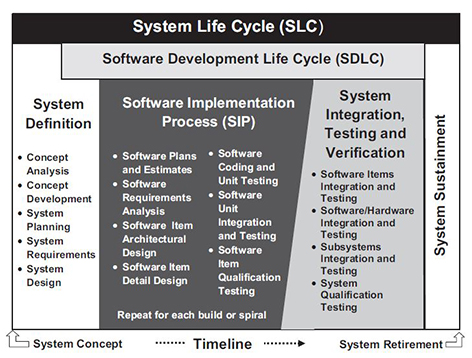
\includegraphics{1.jpg}
\end{document}